%%%%%%%%%%%%%%%%%%%%%%%%%%%%%%%%%%%%%%%%%
% Beamer Presentation
% LaTeX Template
% Version 1.0 (10/11/12)
%
% This template has been downloaded from:
% http://www.LaTeXTemplates.com
%
% License:
% CC BY-NC-SA 3.0 (http://creativecommons.org/licenses/by-nc-sa/3.0/)
%
%%%%%%%%%%%%%%%%%%%%%%%%%%%%%%%%%%%%%%%%%

%----------------------------------------------------------------------------------------
%	PACKAGES AND THEMES
%----------------------------------------------------------------------------------------

\documentclass{beamer}

\mode<presentation> {

% The Beamer class comes with a number of default slide themes
% which change the colors and layouts of slides. Below this is a list
% of all the themes, uncomment each in turn to see what they look like.

%\usetheme{default}
%\usetheme{AnnArbor}
%\usetheme{Antibes}
%\usetheme{Bergen}
%\usetheme{Berkeley}
%\usetheme{Berlin}
%\usetheme{Boadilla}
%\usetheme{CambridgeUS}
%\usetheme{Copenhagen}
%\usetheme{Darmstadt}
%\usetheme{Dresden}
%\usetheme{Frankfurt}
%\usetheme{Goettingen}
%\usetheme{Hannover}
%\usetheme{Ilmenau}
%\usetheme{JuanLesPins}
%\usetheme{Luebeck}
\usetheme{Madrid}
%\usetheme{Malmoe}
%\usetheme{Marburg}
%\usetheme{Montpellier}
%\usetheme{PaloAlto}
%\usetheme{Pittsburgh}
%\usetheme{Rochester}
%\usetheme{Singapore}
%\usetheme{Szeged}
%\usetheme{Warsaw}

% As well as themes, the Beamer class has a number of color themes
% for any slide theme. Uncomment each of these in turn to see how it
% changes the colors of your current slide theme.

%\usecolortheme{albatross}
%\usecolortheme{beaver}
%\usecolortheme{beetle}
%\usecolortheme{crane}
%\usecolortheme{dolphin}
%\usecolortheme{dove}
%\usecolortheme{fly}
%\usecolortheme{lily}
%\usecolortheme{orchid}
%\usecolortheme{rose}
%\usecolortheme{seagull}
%\usecolortheme{seahorse}
%\usecolortheme{whale}
%\usecolortheme{wolverine}

%\setbeamertemplate{footline} % To remove the footer line in all slides uncomment this line
%\setbeamertemplate{footline}[page number] % To replace the footer line in all slides with a simple slide count uncomment this line

%\setbeamertemplate{navigation symbols}{} % To remove the navigation symbols from the bottom of all slides uncomment this line
}

\usepackage{graphicx} % Allows including images
\usepackage{booktabs} % Allows the use of \toprule, \midrule and \bottomrule in tables


%----------------------------------------------------------------------------------------
%	TITLE PAGE
%----------------------------------------------------------------------------------------

\title[Week 3 Coding]{Week 3 Coding: Clustering and Topic Modeling} % The short title appears at the bottom of every slide, the full title is only on the title page

\author{Joseph Denby} % Your name
\institute[] % Your institution as it will appear on the bottom of every slide, may be shorthand to save space
{
Computational Content Analysis \\ % Your institution for the title page
\medskip
%\textit{john@smith.com} % Your email address
}
\date{\today} % Date, can be changed to a custom date

\begin{document}

\begin{frame}
\titlepage % Print the title page as the first slide
\end{frame}

% \begin{frame}
% \frametitle{Overview} % Table of contents slide, comment this block out to remove it
% \tableofcontents % Throughout your presentation, if you choose to use \section{} and \subsection{} commands, these will automatically be printed on this slide as an overview of your presentation
% \end{frame}

\begin{frame}
	\frametitle{Corpus}
	Montag, J. L., Jones, M. N., \& Smith, L. B. (2015). The Words Children Hear. Psychological Science, 26(9), 1489–1496. http://doi.org/10.1177/0956797615594361
	\begin{figure}
		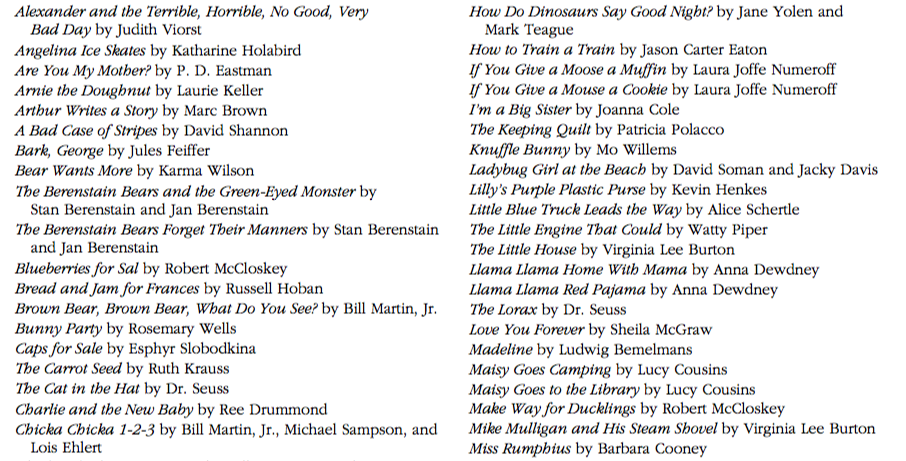
\includegraphics[width=0.9\linewidth]{corpus.png}
	\end{figure}
\end{frame}

\begin{frame}
	\frametitle{Preliminaries}
	Term Frequency-Inverse Document Frequency (tf-idf)	\begin{itemize}
		\item Word frequency scaled by the inverse of document frequency
		\item Used to assess informativeness of word frequency in a document
	\end{itemize}	
\end{frame}


\begin{frame}
	\frametitle{Preliminaries}
	Term Frequency-Inverse Document Frequency (tf-idf)	\begin{itemize}
		\item Word frequency scaled by the inverse of document frequency
		\item Used to assess informativeness of word frequency in a document
	\end{itemize}
	\begin{figure}
		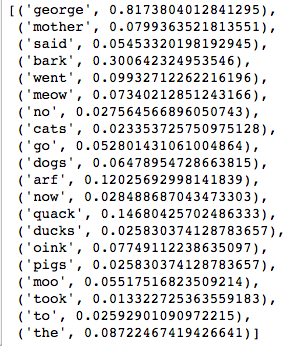
\includegraphics[width=0.4\linewidth]{tfidf.png}
	\end{figure}
\end{frame}

\begin{frame}
	\frametitle{PCA}
	Principle Components Analysis
	\begin{itemize}
		\item {Reduce variance in $n_{docs}$ by $n_{words}$ matrix to 2 dimensions}
		\item Much easier to visualize
	\end{itemize}
\end{frame}

\begin{frame}
	\frametitle{PCA}
	Principle Components Analysis
	\begin{itemize}
		\item {Reduce variance in $n_{docs}$ by $n_{words}$ matrix to 2 dimensions}
		\item Much easier to visualize
	\end{itemize}
	\begin{figure}
		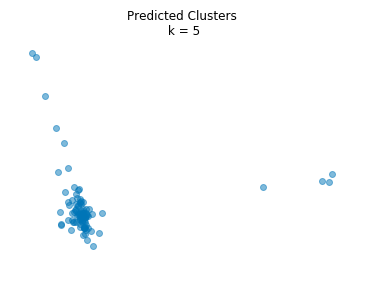
\includegraphics[width=0.6\linewidth]{PCAviz.png}
	\end{figure}
\end{frame}

\begin{frame}
	\frametitle{Flat Clustering}
	\begin{itemize}
		\item Algorithmically group documents according to their tf-idf vectors
		\item Clusters are documents that use similar words similarly 
	\end{itemize}
\end{frame}

\begin{frame}
	\frametitle{Flat Clustering}
		\begin{figure}
			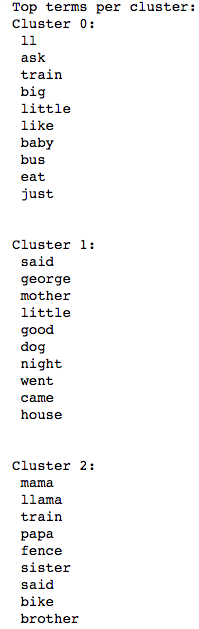
\includegraphics[width=0.2\linewidth]{clusterterms.png}
		\end{figure}
	
\end{frame}
\begin{frame}
	\frametitle{Silhouette}
	Allows us to determine the optimal number of clusters
	\begin{figure}
		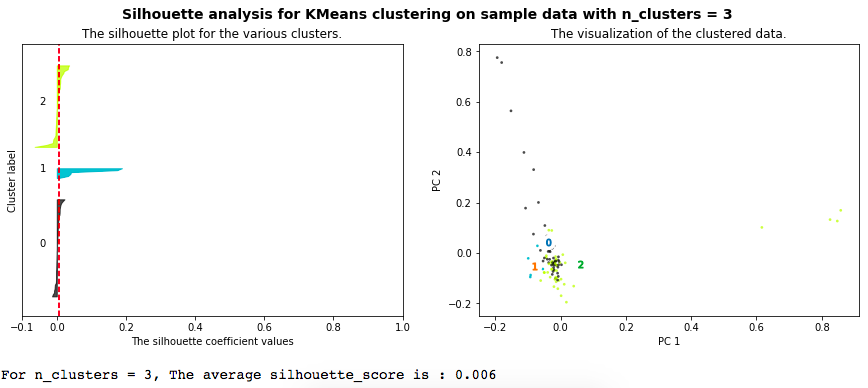
\includegraphics[width=1.0\linewidth]{silhouette3.png}
	\end{figure}
\end{frame}

\begin{frame}
	\frametitle{Silhouette}
	\begin{figure}
		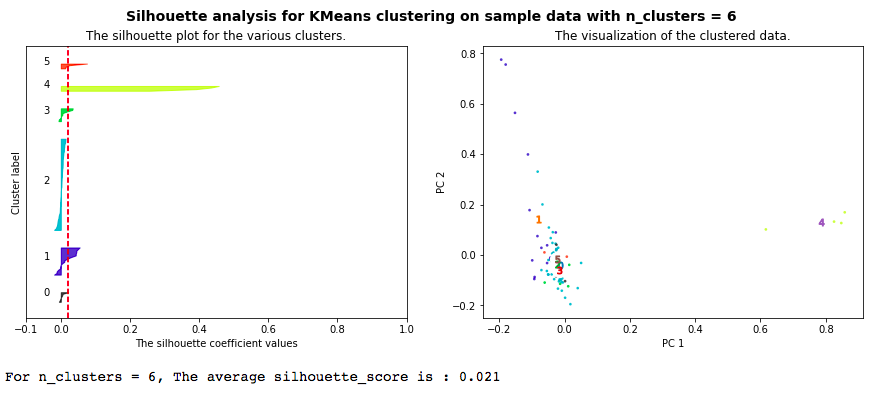
\includegraphics[width=1.0\linewidth]{silhouette6.png}
	\end{figure}
	No obvious clustering to the books\\
	Hard to determine given outliers
\end{frame}

\begin{frame}
	\frametitle{Hierarchical Clustering}
	A different approach that creates clusters at various points of resolution
	\begin{figure}
		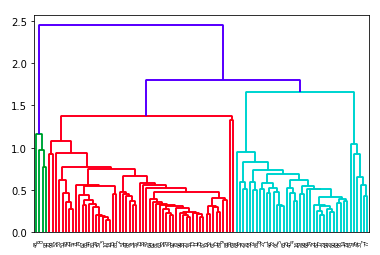
\includegraphics[width=.9\linewidth]{uncutdendro.png}
	\end{figure}
\end{frame}

\begin{frame}
	\frametitle{Hierarchical Clustering}
	A different approach that creates clusters at various points of resolution
	\begin{figure}
		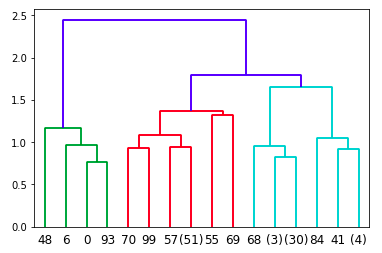
\includegraphics[width=.9\linewidth]{cutoffdendro.png}
	\end{figure}
\end{frame}

\begin{frame}
	\frametitle{Topic Modeling}
	Assign words to topics based on frequency and co-occurence
	\begin{figure}
		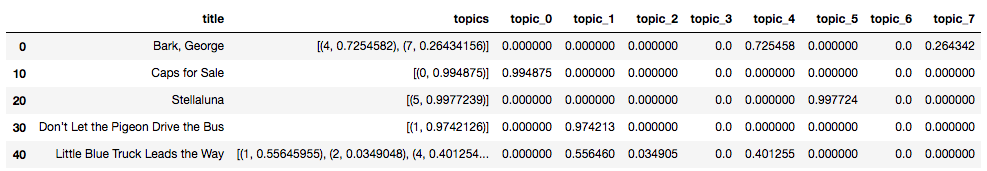
\includegraphics[width=1.0\linewidth]{ldatable.png}
	\end{figure}
\end{frame}

\begin{frame}
	\frametitle{Topic Modeling}
	Each topic is a probability distribution of all words in the corpus.
	\begin{figure}
		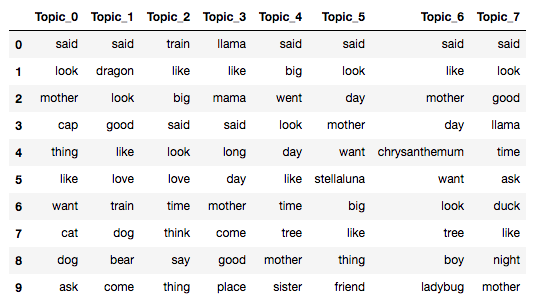
\includegraphics[width=1.0\linewidth]{ldawords.png}
	\end{figure}
\end{frame}

\begin{frame}
	\frametitle{Topic Modeling}
	Each document is a probability distribution of all topics.
	\begin{figure}
		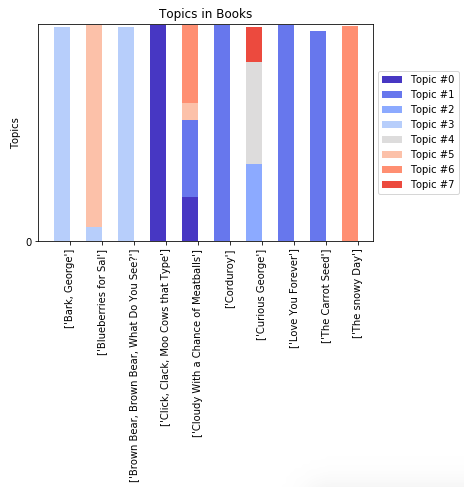
\includegraphics[width=0.64\linewidth]{topicsbarchart.png}
	\end{figure}
\end{frame}

\begin{frame}
	\frametitle{Topic Modeling}
	Each document is a probability distribution of all topics.
	\begin{figure}
		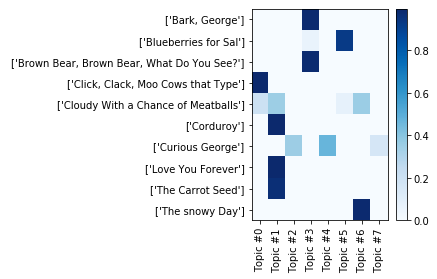
\includegraphics[width=0.9\linewidth]{ldaheatmap.png}
	\end{figure}
\end{frame}
\begin{frame}
	\frametitle{Topic Modeling}
	Can adjust the topic modeling algorithm parameters as well
	\begin{itemize}
		\item $\alpha$ - sparsity of document-topic loadings
		\item $\eta$ - sparsity of topic-word loadings
	\end{itemize}
\end{frame}
\begin{frame}
	\frametitle{Topic Modeling}
	\begin{figure}
		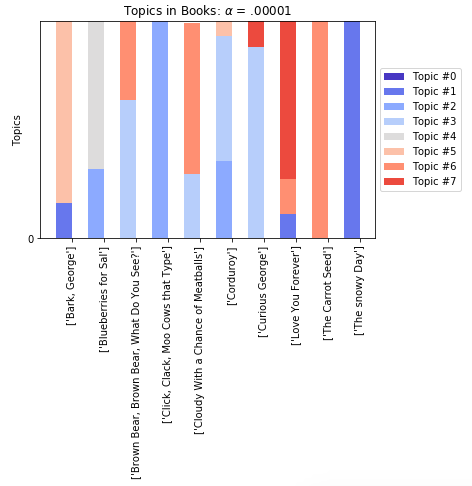
\includegraphics[width=.64\linewidth]{lowalpha.png}
	\end{figure}
\end{frame}
\begin{frame}
	\frametitle{Topic Modeling}
	\begin{figure}
		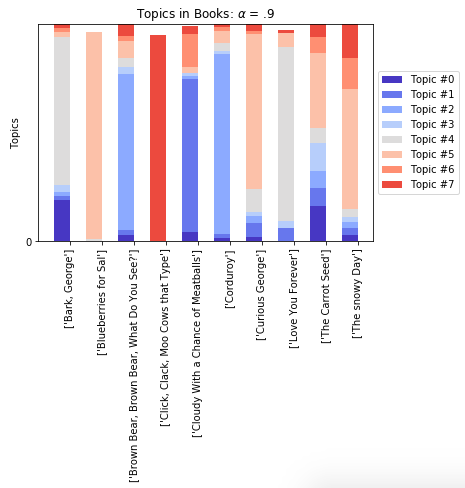
\includegraphics[width=.64\linewidth]{highalpha.png}
	\end{figure}
\end{frame}
\begin{frame}
	\frametitle{Topic Modeling}
	\begin{figure}
		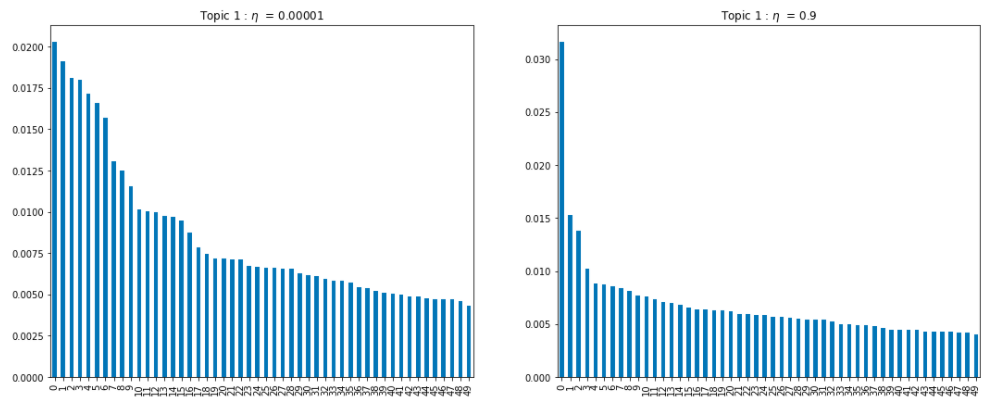
\includegraphics[width=1\linewidth]{etadem.png}
	\end{figure}
\end{frame}
\end{document}